% !TEX encoding = IsoLatin2  % notwendige Zeile f"ur Mac-Benutzer (muss als Kommentar stehen); Windows-Benutzer k"onnen die Zeile l"oschen.

% LaTeX-Vorlage Version 3.1,  Juli 2011
% erstellt von Dr. Andreas Drauschke (andreas.drauschke@technikum-wien.at) und Dr. Susanne Teschl (susanne.teschl@technikum-wien.at)
% geringf"ugig adaptiert von Harald Stockinger (harald.stockinger@technikum-wien.at)

 
\documentclass[a4paper,bibtotoc,oneside]{scrbook} 
% F"ur kurze Arbeiten w"are auch die Dokumentklasse "scrartcl" ausreichend. In diesem Fall ist "section" die h"ochste Ebene ("chapter" gibt es dann nicht).
% \documentclass[a4paper,bibtotoc,oneside]{scrartcl}

%\usepackage{cclicenses}

% verlinkte Querverweise im pdf
\usepackage{hyperref}

% deutsche Anpassungen
\usepackage[ansinew]{inputenc}
\usepackage[T1]{fontenc}
\usepackage[ngerman]{babel}

% mathematische Symbole
\usepackage{amsmath,amssymb,amsfonts,amstext}

% Kopfzeilen frei gestaltbar
\usepackage{fancyhdr}
\lfoot[\fancyplain{}{}]{\fancyplain{}{}}
\rfoot[\fancyplain{}{}]{\fancyplain{}{}}
\cfoot[\fancyplain{}{\footnotesize\thepage}]{\fancyplain{}{\footnotesize\thepage}}
\lhead[\fancyplain{}{\footnotesize\nouppercase\leftmark}]{\fancyplain{}{}}
\chead{}
\rhead[\fancyplain{}{}]{\fancyplain{}{\footnotesize\nouppercase\sc\leftmark}} 

% Farben im Dokument m"oglich
\usepackage{color}

% Schriftart Helvetica
\usepackage{helvet}
\renewcommand{\familydefault}{cmss} 

% Graphiken einbinden: hier f"ur pdflatex
\usepackage[pdftex]{graphicx}

\usepackage{array}

% H"ohe und Breite des Textk"orpers etwas gr"osser definieren
\setlength{\textheight}{225mm}
\setlength{\textwidth}{1.05\textwidth}

% weniger Warnungen wegen "uberf"ullter Boxen
\tolerance = 9999
\sloppy

% Anpassung einiger "Uberschriften 
\renewcommand\figurename{Abbildung}
\renewcommand\tablename{Tabelle}

\begin{document}

% Kopf- und Fusszeilen initiieren
\pagestyle{fancy}
\pagenumbering{Alph}

% Deckblatt:
\thispagestyle{empty}
\begin{picture}(0,0)
\color{white}\sffamily
\put(-101,-749){
\includegraphics[width=1.002\paperwidth, height=\paperheight]{BM_2011.pdf}}
\put(220,-670){
\includegraphics[width=0.5\textwidth]{FHTW_Logo_4c.pdf}}
\put(-30, -20){\bfseries\huge BACHELORARBEIT}
% Titel des Studienganges einf"ugen:
\put(-30,-50){\Large im Studiengang Bachelor Informatik}
% Titel der Arbeit einf"ugen:
% Die Minipage wird gesetzt, damit auch mehrzeilige Titel m"oglich werden.
\put(-32,-150){
\begin{minipage}{14cm}
\bfseries\huge Accessibility im Modern Web
\end{minipage}
}
% Name der Autorin/des Autors eingeben:
\put(-30,-250){\large Ausgef"uhrt von: Bernhard Posselt}
% Personenkennzeichen der Autorin/des Autors eingeben:
\put(-30,-270){\large Personenkennzeichen: 1010257029}
% Name der Begutachterin/des Begutachters eingeben:
\put(-30,-310){\large Begutachter: Dipl.-Ing. Mag. Dr. Michael Tesar}
\put(-30,-350){\large Wien, \today} % das Datum des letzten Kompilierens wird automatisch eingesetzt
\color{black}
\end{picture}

\newpage


\section*{Eidesstattliche Erkl"arung}\thispagestyle{empty}
\glqq Ich erkl"are hiermit an Eides statt, dass ich die vorliegende Arbeit selbst"andig angefertigt habe. 
Die aus fremden Quellen direkt oder indirekt "ubernommenen Gedanken sind als solche kenntlich gemacht. 
Die Arbeit wurde bisher weder in gleicher noch in "ahnlicher Form einer anderen Pr"ufungsbeh"orde vorgelegt
und auch noch nicht ver"offentlicht. Ich versichere, dass die abgegebene Version jener im Uploadtool entspricht.\grqq\\[5\baselineskip]
\rule{5cm}{0.2pt}\hfill\rule{5cm}{0.2pt}\\
\phantom{Datum }Ort, Datum\hfill Unterschrift\hspace{15mm}

\newpage


\section*{Kurzfassung}\thispagestyle{empty}
In dieser Arbeit wird ein "Uberblick "uber moderne Web-Technologien im Bereich
Accessibility gegeben. Immer mehr "offentliche Einrichtungen stellen im Rahmen des \emph{e-governments} heutzutage einen Zugang zu wichtige Informationen und Services im Web bereit. Dadurch muss dieser Zugang universell erreichbar und nutzbar sein. Um eine L"osung f"ur dieses Problem zu finden, wird ein Blick auf die Empfehlungen der W3C geworfen. Auch auf neuere Techniken wie ARIA, die erst in einer Candidate Recommendation vorhanden sind, werden eingangen. Das Ziel dieser Arbeit sollte ein guten "Uberblick "uber den heutigen Stand bieten und die Vorteile der Nutzung von Accessibility Methoden hervorstreichen. 
\vfill
\paragraph*{Schlagw"orter:} Accessibility, Web, ARIA, HTML5


\newpage

\section*{Abstract}\thispagestyle{empty}
This thesis will present an overview over accessibility techniques used in the
modern web. Over the last years the usage of the web to present and
access information and services of public institutions has increased
dramatically. This requires the services and information to be accessible for
every citizen. To find a solution for this problem, this thesis will look at
the W3C's recommendations and guidelines. Also newer techniques like ARIA
and the role attribute which are currently in the Candidate Recommendation
phase will be part of it. The goal of this thesis is to present the current
status of accessibility in the web and to show the advantages of using these
techniques.
\vfill
\paragraph*{Keywords:} Accessibility, Web, ARIA, HTML5
\newpage

%\section*{Danksagung}
%\thispagestyle{empty}
%Text Text Text Text Text Text Text Text Text Text Text Text Text Text Text Text
%\newpage

\tableofcontents\thispagestyle{empty}
\newpage

\pagenumbering{arabic}
\setcounter{page}{1}

% Falls die Kapitel"uberschriften zu lang f"ur die Kopfzeile oder das Inhaltsverzeichnis sind, so erzielt man
% dort Kurzformen der Kapitelbezeichnungen mittels:
% \chapter[Kurzform]{Lange "Uberschrift}
\chapter{Einf"uhrung}
Das Web spielt im "offentlichen Bereich eine immer gr"o"sere Rolle: Viele
Services und Informationen werden bereits "uber eigens daf"ur erstellte Portale angeboten. Daraus folgt, dass das "offentliche Leben immer st"arker mit dem Web verwoben wird. Wie auch bei anderen "offentlichen Einrichtungen muss ein universeller Zugang f"ur alle B"urger erm"oglicht werden, auch f"ur jene, die mit k"orperlichen Einschr"ankungen oder Lernschwierigkeiten leben m"ussen, z. B. Blinde oder Personen mit eingeschr"ankten motorischen F"ahigkeiten. Solange dies nicht vollst"andig m"oglich ist muss als Ersatz eine zus"atzliche Einrichtung bereitstehen, die die gleichen M"oglichkeiten bietet \cite[S. 8]{understand_acc}. Es steht also auch im wirtschaftlichen Interesse "offentlicher Einrichtungen, ihre Services und Informationen barrierefrei anzubieten. 

Dadurch, dass diese Gruppe eine Minorit"at in der Bev"olkerung ausmacht und noch dazu das Web auf andere Weise verwendet als nicht eingeschr"ankte Personen - z. B. blinde Personen verwenden Screen-Reader oder Braillen - muss oft ein zus"atzlicher Aufwand bei der Erstellung von Webseiten betrieben werden. Ja "ofters wird sogar ganz darauf vergessen.\cite[S. 7]{mod_software} Roman Mauerhofer erfasst dieses Problem mit einem sehr treffenden Vergleich: \glqq Es ist beispielsweise so, als ob ein Architekt bei der Planung eines Bahnhofes den Einbau von Aufz"ugen vergisst.\grqq  \cite[S. 7]{mod_software}

Diese Gruppe macht jedoch nicht einen ganz so geringen Prozentanteil in der Bev"olkerung aus wie "ofters gedacht. Laut einem Bericht des U.S. Census Bureau aus dem Jahre 2000 leben alleine in den USA ca. 49.7 Millionen Menschen mit k"orperlichen Einschr"ankungen und Lernschwierigkeiten (entspricht ca. 20\% der amerikanischen Bev"olkerung), davon haben 42,9 Millionen eine schwere Einschr"ankung und 6,8 Millionen haben eine so gravierende Einschr"ankung, dass sie Hilfe in ihrem allt"aglichem Leben brauchen \cite[S. 1]{us_cens}. Laut der World Health Organization wird die weltweite Anzahl von Personen mit k"orperlichen oder geistigen Einschr"ankungen auf 500 bis 600 Millionen Menschen gesch"atzt \cite{who_dis}.

Auch die UN erkennt eine immer gr"o"ser werdende Wichtigkeit in der angemessenen Bereitstellung von Informationen f"ur k"orperlich eingeschr"ankten Personen und Personen mit Lernschwierigkeiten. Dies spiegelt sich in der \glqq UN Convention of Rights for Persons with Disabilities\grqq wider, welche am 30. M"arz 2007 unterzeichnet wurde. Sie erhielt die \glqq meisten Unterschriften an einem Er"offnungstag in der Geschichte der UN Konventionen\grqq \cite{un_disabilities}. 

Jedoch kann es nicht nur aus den oben genannten Gr"unden erforderlich sein,
einen barrierefreien Zugang bereitzustellen, sondern sogar gesetzlich
vorgeschrieben. In den USA beispielsweise, gibt es daf"ur ein eigenes
Gesetz, den \glqq Americans with Disabilities Act\grqq aus dem Jahre 1990 (ADA) und den Abschnitt 508 aus dem \glqq Rehabilitation Act\grqq (1973) \cite[S. 288-289]{achieving_web_acc}. Auch in Europa sind einige "ahnliche Regelungen vorhanden \cite[S. 7]{mod_software} doch eines haben sie beide gemeinsam: Sie basieren alle zu einem gro"sen Teil auf den Richtlinien der WAI (Web Accessibility Initiative), den WCAG (Web Content Accessibility Guidelines) \cite[S. 289]{achieving_web_acc} \cite[S. 7]{mod_software}.

\section{Problemstellung}
Nicht nur in der EU wird Accessibility k"unftig eine gr"o"sere Rolle spielen \cite[Abschnitt EU]{w3c_pol} sondern auch in der Privatwirtschaft. F"ur viele ProgrammiererInnen stellt jedoch die Implementation und das Testen von Accessibility Techniken einen nicht zu untersch"atzenden Mehraufwand dar \cite[S. 27]{understand_acc} und dadurch werden ihnen, selbst wenn sie es umsetzen wollen, oft Steine in den Weg gelegt. Dies erfolgt h"aufig in der Nennung nicht zu Ende gedachter Argumenten wie \glqq Barrierefreiheit bringt keine Vorteile\grqq \cite[S. 28]{understand_acc} oder \glqq Behinderte geh"oren nicht zu unserer Zielgruppe\grqq \cite[S. 31]{understand_acc}.

Ein weiteres Problem ist die geringe Verbreitung der Standards, welche aus einer globalen Studie der United Nations im Jahre 2006 hervorging\cite{acc_report}: Nur drei von 100 getesteten Seiten erhielten die Bestnote \cite [S. 7]{acc_report}. Dies ist unter anderem auf ein Fehlen folgender Punkte zur"uckzuf"uhren: Achtsamkeit (Vergessen oder "Ubersehen von Fehlern und Problemen im Bereich Accessibility), Bildung (Accessibility-Techniken sind unbekannt) und Tool Support (Techniken werden nicht von Programmierwerkzeugen unterst"utzt) \cite[S. 13]{tool_acc}.


\section{L"osungsansatz}
In dieser Bachelorarbeit soll ein genereller "Uberblick "uber die bestehenden und einsetzbaren Techniken gegeben werden, die hilfreich f"ur die Verbesserung im Bereich Accessibility im Modern Web sind. 

Dazu soll ein eine "Ubersicht "uber die vom W3C bereitgestellten Spezifikationen, wie den WCAG 1.0 \cite{wcag1}, WCAG 2.0 \cite{wcag2} und ARIA \cite{aria} gegeben werden und auf die Unterschiede von WCAG 1.0 und WCAG 2.0 eingegangen werden.

Zus"atzlich soll kurz auf die verschiedenen Arten von Einschr"ankungen eingegangen werden und die Probleme und verwendeten Hilfsger"ate aufgezeigt werden.

\section{Aufbau}
In Kapitel 2 wird ein kurzer "Uberblick "uber die h"aufigsten Einschr"ankungen gegeben und erkl"art, welche assistiven Technologien verwendet werden, um k"orperlich eingeschr"ankten Personen und Personen mit Lernschwierigkeiten beim Zugriff auf das Web zu helfen. Die soll veranschaulichen, warum man Webseiten f"ur diese Ger"ate optimieren soll.

In Kapitel 3 wird auf die Richtlinien des W3C, die WCAG, eingegangen und die Entwicklung und Unterschiede zwischen der Version 1 und Version 2 betrachtet.

In Kapitel 4 wird ein Blick auf ARIA geworfen und der Sinn und Einsatzzweck von verschiedenen Attributes und Roles wird erl"autert.

In Kapitel 5 wird eine Zusammenfassung der jetzigen Situation und ein Ausblick "uber kommende Richtlinien gegeben, welche sich noch im \emph{Draft} Status befinden.

\section{Begriffe}
Da der Begriff \glqq Menschen mit geistigen Behinderungen/Einschr"ankungen\grqq auf negative Weise verstanden werden kann, wird in dieser Arbeit stattdessen der Begriff \glqq Menschen mit Lernschwierigkeiten\grqq  verwendet. Dies ist gleich zu setzen mit den Abschnitten F70-F79 im ICD-10 \cite{icd10}. Dazu z"ahlen unter anderem Menschen mit Konzentrationsschw"achen.


Der Begriff \glqq Menschen mit k"orperliche Einschr"ankung\grqq wird synonym f"ur Personen verwendet, welche durch eine Verletzung, Nichtfunktion oder Amputation eines K"orperteiles Einschr"ankungen im t"aglichen Leben erfahren m"ussen. Dazu z"ahlen unter anderem Menschen mit Sehschw"achen oder Blindheit und Menschen mit einer Fehlbildung der Finger oder den H"anden.

\chapter{Arten von k"orperlichen Einschr"ankungen oder Lernschwierigkeiten
 und assistive Technologien}

\section{Personen mit Sehschw"achen}
Die Anzahl blinder Personen allein in den USA wird auf eine Million Personen und weltweit auf 38 Millionen Personen gesch"atzt\cite[S. 1]{screen_read}.  Als offiziell blind gilt eine Person, wenn sie unter 2\% auf dem besseren der zwei Augen wahrnimmt \cite[S. 12]{understand_acc}. 

Jedoch umfasst diese Kategorie nicht nur blinde Personen sondern auch Personen mit teilweisen Sehschw"achen: Nimmt jemand auf dem besten Auge weniger als 30\% wahr f"allt er/sie bereits unter diese Kategorie\cite[S. 12]{understand_acc}. In "Osterreich betr"agt die Anzahl der Personen mit Sehschw"achen rund 318.000 Personen, das entspricht 3,9\% der Bev"olkerung \cite[S. 13]{stat_austria}. Weltweit wird gesch"atzt, dass mindestens sechs Millionen Personen von so schweren Sehschw"achen betroffen sind, dass f"ur sie die Nutzung eines Computerbildschirmes unm"oglich ist\cite[S. 249]{screen_read_frust}.

Personen mit Sehschw"achen haben die gr"o"sten Probleme nicht mit den Eingabeger"aten - die meisten Nutzer beherrschen Tippen ohne das auf die Tastatur zu schauen - sondern mit den Ausgabeger"aten. Die am meisten genutzten assistiven Technologien in diesem Umfeld sind Screen-Reader und Braillen (siehe \ref{Abb1}). Braillen und andere in Hardware umgesetzte Technologien sind jedoch meistens sehr teuer, da sie nur von einem geringen Prozentsatz der Bev"olkerung ben"otigt werden und deren Erlernung, beispielsweise die der Braillenschrift, aufwendig und dementsprechend wenig verbreitet ist\cite[S. 249-250]{screen_read_frust}.
Zus"atzlich besteht die Braille aus vielen kleinen, mechanischen Teilen und ist deshalb besonders verschlei"sanf"allig \cite[S. 11]{barr_webd}.

\begin{figure}[braille]
\centering
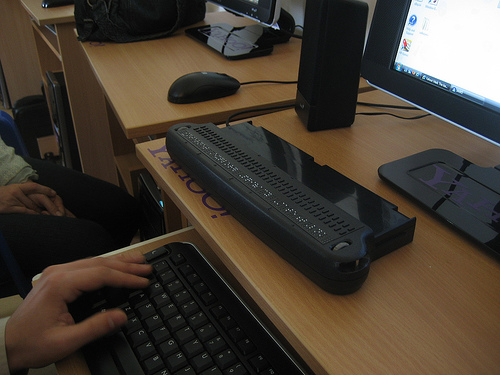
\includegraphics[width=75mm]{braille}
\caption[Beschriftung eines Buchr"uckens.]{Beispiel einer Braille (\copyright  Philip Tellis, Creative Commons BY-SA)}\label{Abb1}
\end{figure}

Deshalb ziehen die Meisten auf Software basierende L"osungen vor, was dem Screen-Reader zu einer h"oheren Popularit"at verhilft\cite[S. 249-250]{screen_read_frust}. Ein Screen-Reader liest dem/der NutzerIn die Inhalte auf dem Bildschirm vor. Dies kann f"ur sehende Personen als st"orend empfunden werden, blinde Personen sind jedoch st"arker auf auditive Reize ausgerichtet und kommen dementsprechend besser damit klar\cite[S. 13]{barr_webd}. Bestimmte Screen-Reader wie GNOME Orca \cite{orca} sind sogar frei f"ur jeden verf"ugbar. 
F"ur diese Personen muss beim Erstellen von Websiten besonders folgendes beachtet werden: semantisch korrekter und sauberer HTML Code, der den Inhalt vom Layout trennt.\cite[S. 13-15]{barr_webd}

\section{Personen mit H"orschw"achen}
Alleine in "Osterreich befinden sich ca. 202.000 Personen (2,5\% der Bev"olerkung) mit eingeschr"ankter H"orf"ahigkeit. Personen mit schweren H"orschw"achen machen rund 2000 Personen aus \cite[S. 13-14]{stat_austria}. Die gr"o"sten Probleme entstehen f"ur diese Gruppe, wenn eine Website eine bestimmte Information nur "uber akustische Signale wiedergibt. Dies kann z. B. ein einfaches Video oder ein Podcast sein, oder ein Warnsignalton. \cite[S. 17]{barr_webd}\cite[S. 20]{understand_acc}

F"ur diese Personen muss man vor allem folgendes beachten: Bereitstellung von Untertiteln bei Videos oder Transkriptionen von Podcasts und Verzichten auf \glqq audio-only\grqq L"osungen. Das Anbieten von Videos mit Geb"ardensprache kann n"utzlich sein, stellt jedoch einen hohen Aufwand dar, den jeder/jede AuftraggeberIn selbst f"ur sich entscheiden muss. \cite[S. 17]{barr_webd}\cite[S. 20]{understand_acc}

\section{Personen mit motorischen Schw"achen}
Diese Gruppe macht laut dem U.S. Census Report 21.2 Millionen Personen aus. Das
sind ca. 8.2 Prozent der Bev"olkerung der USA \cite[S. 1]{us_cens}. In "Osterreich betr"agt deren Anzahl 1 Million bzw. 13\% der Bev"olkerung \cite[S. 12]{stat_austria}. Probleme mit der Computerbenutzung treten vor allem dann auf, wenn Personen ihre H"ande nur eingeschr"ankt oder gar nicht verwenden k"onnen, beispielsweise Querschnittsgel"ahmte. F"ur diese muss eine alternative Steuerung des Computers angeboten werden. Darunter fallen z. B. Ger"ate, welche es den NutzerInnen erlauben, den Computer mit ihrer Zungenspitze zu bedienen.\cite[S. 15-16]{barr_webd}

Diese Art der Bedienung ist offensichtlich aufw"andiger und schwieriger und profitiert deshalb am Meisten von einer klaren Struktur der Seite und einer guten Bedienbarkeit mit der Tastatur.\cite[S. 15-16]{barr_webd}\cite[S. 18]{understand_acc}

\section{Personen mit Lernschwierigkeiten}
Diese Gruppe macht laut dem U.S. Census Report 12.4 Millionen Personen aus. Das
sind ca. 4.8 Prozent der Bev"olkerung der USA \cite[S. 1]{us_cens}. Jedoch geh"oren zu dieser Gruppe auch Analphabeten, welche etwa in Deutschland ca. vier Millionen Personen ausmachen (ca. 6.3\% der deutschen Bev"olkerung) \cite[S. 19]{understand_acc}. In "Osterreich sind 85.000 Personen bzw. 1\% der Bev"olkerung von Lernschwierigkeiten betroffen \cite[S. 14]{stat_austria}.

Diese Personen haben vor allem Probleme mit zu komplizierten S"atzen oder einer fehlenden Struktur der Seite. Dadurch profitieren sie am Meisten durch: einfache und kurze S"atze, gute Strukturierung, Einsetzen von Bildern und Anbieten von einer Methode zum Vorlesen von Texten, was auch \glqq Text-to-Speech\grqq genannt wird. \cite[S. 18-19]{barr_webd}\cite[S. 19]{understand_acc}

\chapter{WCAG}
Die WCAG (Web Content Accessibility Guidelines) sind ein Dokument, welches vom W3C herausgegeben wurde um Webseiten auch f"ur k"orperlich eingeschr"ankte Personen oder Personen mit Lernschwierigkeiten zug"anglich zu machen. Jedoch bringt das Befolgen dieser Richtlinien auch zus"atzliche Vorteile f"ur andere NutzerInnen, z. B. Personen die mit mobilen Ger"aten oder mit anderen durch Form oder Einsatzgebiet eingeschr"ankten Plattformen auf das Web zugreifen. \cite[Abschnitt Abstract]{wcag1}


\section{WCAG Version 1.0}
Die Version 1.0 des Dokumentes wurde im Jahre 1999 finalisiert und beinhaltet 14 Richtlinien, welche jeweils Empfehlungen f"ur WebentwicklerInnen enthalten. Diese Empfehlungen enthalten Unterpunkte, so genannte Checkpoints, die wiederum mit einer Priorit"at gekennzeichnet sind. \cite[Abschnitt Abstract]{wcag1}
F"ur eine bessere Gegen"uberstellung dieser Kriterien mit den WCAG 2.0 wird versucht, diese 14 Richtlinien der WCAG 1.0 in die gleiche Struktur wie die der WCAG 2.0 zu bringen.

\subsection{Success Criteria}
Die Kriterien anhand derer man die erfolgreiche Umsetzung der Richtlinien pr"ufen kann werden in drei verschiedene Kategorien aufgeteilt: must, should und may Kriterien, sprich Kriterien die erf"ullt sein m"ussen, sollen und k"onnen. Anhand der Erf"ullung dieser Kritieren lassen sich nun folgende Konformit"atslevel definieren: \cite[Abschnitt 4]{wcag1}

\begin{itemize}
\item \emph{A}: Alle mit Priorit"at 1 angef"uhrten Kritierien sind umgesetzt
\item \emph{AA}: Alle mit Priorit"at 1 und 2 angef"uhrten Kritierien sind umgesetzt
\item \emph{AAA}: Alle mit Priorit"at 1, 2 und 3 angef"uhrten Kritierien sind umgesetzt
\end{itemize}

Die deutsche BITV (Barrierefreie Informationstechnologie Verordnung), welche im \emph{Bundesgesetz zur Gleichstellung behinderter Menschen} festgeschrieben ist, baut z. B. auf diesen Kriterien auf. Will man die BITV komplett erf"ullen, m"ussen sowohl die Kriterien der Stufe 1, als auch die der Stufe 2 komplett erf"ullt werden, was einer Mindeststufe des Konformit"atslevels AA entspricht. \cite[S. 38-39]{barr_webd}

\subsection{Wahrnehmbarkeit}
Unter die Kategorie Wahrnehmbarkeit fallen folgende Richtlinien: 

\begin{itemize}
\item Visuelle oder auditive Elemente sollen eine textbasierte Alternative besitzen\cite[Abschnitt 6.1]{wcag1}
\item Der Sinn des Inhalts sollte nicht nur von der Farbe abh"angig sein \cite[Abschnitt 6.2]{wcag1}
\end{itemize}

\subsubsection{Visuelle oder auditive Elemente sollen eine textbasierte Alternative besitzen}
Diese Richtlinie bezieht sich vor allem auf Personen mit Sehschw"achen und besagt, dass f"ur alle eingesetzten visuellen oder auditiven Elemente wie Bilder, Videos oder Kl"ange eine dementsprechende Alternative vorhanden sein soll. Dies kann z. B. erreicht werden, indem <img> Elemente immer ein \emph{alt} Attribut besitzen oder Videos/Kl"ange mit einem beschreibenden Text oder Transkription versehen sind. Von den Kritieren, die  zur Erf"ullung dieser Richtlinien aufgez"ahlt sind, sind vier von f"unf der Priorit"at 1 zuzuordnen. \cite[Abschnitt 6.1]{wcag1}

\subsubsection{Der Sinn des Inhalts sollte nicht nur von der Farbe abh"angig sein}
Diese Richtlinien bezieht sich vor allem Personen mit Rot-Gr"un Blindheit oder Personen, deren Monitor keine Farben ausgeben kann \cite[S. 41]{barr_webd}. Dazu muss sicher gestellt werden, dass ein ausreichender Kontrast zwischen Hintergrund und Inhalt gew"ahrleistet ist (Priorit"at 2), und dass alle Informationen, die durch Farbe transport werden, auch ohne Farbe verstanden werden k"onnen (Priorit"at 1) \cite[Abschnitt 6.1]{wcag1}


\subsection{Bedienbarkeit}
Unter die Kategorie Bedienbarkeit fallen folgende Richtlinien: 

\begin{itemize}
\item Elemente, die von der Zeit abh"angen, sollen stoppbar oder pausierbar sein \cite[Abschnitt 6.7]{wcag1}
\item Eingebettete Objekte sollen zug"anglich sein\cite[Abschnitt 6.8]{wcag1}
\item Das Userinterface soll auch auf anderen Plattformen bedienbar sein\cite[Abschnitt 6.9]{wcag1}
\item Eine gut strukturierte Navigation soll verf"ugbar sein\cite[Abschnitt 6.13]{wcag1}
\end{itemize}

\subsubsection{Elemente, die von der Zeit abh"angen, sollen stoppbar oder pausierbar sein}
Diese Richtlinie bezieht sich vor allem auf Personen mit Lern- und Konzentrationsschwierigkeiten und Personen mit k"orperlichen Einschr"ankungen. Es kann sein, dass auf einer Webseite z. B. sich schnell bewegende oder blinkende Elemente vorhanden sind. Diese sind f"ur Personen, welche z. B. Einschr"ankungen in der Beweglichkeit ihrer H"anden haben besonders schwer zu treffen. F"ur Personen mit Konzentrations- und Lernschwierigkeiten oder Sehschw"achen k"onnen diese Texte sogar unlesbar sein, z. B. Screen-Reader k"onnen sich bewegende Texte nicht lesen. \cite[Abschnitt 6.7]{wcag1}
Au"serdem k"onnen Blinkende Elemente oder Flickern des Bildschirms, z. B. durch neu laden der Seite bei Epileptikern Anf"alle verursachen.
Diese Elemente sollten daher vermieden werden oder wenn verwendet pausierbar oder abschaltbar sein. \cite[S. 45]{barr_webd}

Weiters sollte sich die Seite auch nicht automatisch neu laden, da Screen-Reader oft mitten im Lesen abbrechen und den Text von neuem vorlesen. NutzerInnen dieser Ger"ate k"onnen so beispielsweise komplett die Orientierung verlieren. \cite[S. 45]{barr_webd}

\subsubsection{Eingebettete Objekte sollen zug"anglich sein}
Um die Zug"anglichkeit der ganzen Seite zu gew"ahrleisten, m"ussen auch einzelne, eingebettete Objekte wie Java Applets oder Flash Container zug"anglich gestaltet sein. Ist dies nicht m"oglich, muss eine Alternative angeboten werden. \cite[Abschnitt 6.8]{wcag1}

\subsubsection{Das Userinterface soll auch auf anderen Plattformen bedienbar sein}
NutzerInnen verwenden die Seite auch oft auf anderen Ger"aten, wie z. B. Mobiltelefonen oder Terminals. Da diese Ger"ate oft verschiedene Eingabemethoden unterst"utzen, muss die Seite auch dahingehend optimiert werden. Dies umfasst z. B. die Bereitstellung eines funktionierenden Tabindexes oder Shortcuts f"ur oft verwendete Links. Desweiteren sollen Eingabespezifische Event-Handler wie z. B. \emph{onkeypress} vermieden vermieden und versucht werden, diese stattdessen logisch anzuordnen. \cite[Abschnitt 6.9]{wcag1}

\subsubsection{Eine gut strukturierte Navigation soll verf"ugbar sein}
Diese Richtlinie betrifft vor allem Menschen mit Lern- und Konzentrationsschwierigkeiten und Personen mit Sehschw"achen. Eine einfache Navigation kann die Benutzung mit dem Screen-Reader angenehmer gestalten und die Orientierung zu verbessern. Dazu geh"oren unter anderem das Vorhandensein einer \glqq Site-Map \grqq und konsistent Navigationselementen: z.B. m"ussen die Ziele eines Links klar ersichtlich sein und "Uberschriften m"ussen unterscheidbar von anderen "Uberschriften sein. \cite[Abschnitt 6.13]{wcag1}
Von diesen Ma"snahmen k"onnen auch andere NutzerInnen profitieren, da sie den gesuchten Inhalt auf der Seite besser finden k"onnen \cite[S. 52]{barr_webd}.

\subsection{Verst"andlichkeit}
Unter die Kategorie Verst"andlichkeit fallen folgende Richtlinien: 

\begin{itemize}
\item Verwendete Hauptsprache und Fremdsprachen sollen gekennzeichnet werden\cite[Abschnitt 6.4]{wcag1}
\item Information zu Kontext und Orientierung soll verf"ugbar sein\cite[Abschnitt 6.12]{wcag1}
\item Der Inhalt der Seite soll einfach und gut verst"andlich sein\cite[Abschnitt 6.14]{wcag1}
\end{itemize}

\subsubsection{Verwendete Hauptsprache und Fremdsprachen sollen gekennzeichnet werden}
Ein Vorhandensein von Sprachinformationen f"ur bestimmte Teile des Textes oder Abk"urzungen erm"oglicht es z. B. Screen-Readern, die Information in der korrekten Sprache auszugeben. Dazu soll das \emph{lang} Attribut verwendet werden, was zu einer der wichtigsten Kriterien z"ahlt (Priorit"at 1). F"ur Abk"urzung gibt es das \emph{<akronym>} und \emph{<abbr>} Element.
Nat"urlicherweise soll auch die Hauptsprache der Webseite mit angegeben werden.\cite[Abschnitt 6.4]{wcag1}

\subsubsection{Information zu Kontext und Orientierung soll verf"ugbar sein}
Diese Richtlinie beschreibt vor allem den korrekten Umgang mit Frames und die korrekte Gruppierung von Elementen \cite[S. 50]{barr_webd}. Frames sollen identifizierbar sein und deren Sinn soll f"ur den/die BenutzerIn klar sein. Daf"ur werden die beiden Attribute \emph{title} und \emph{longdesc} vorgeschlagen. Des weiteren sollen verwandte Informationen und Links mit den daf"ur vorgesehen HTML Elementen gruppiert werden, z. B. mit \emph{<fieldset>} und \emph{<optgroup>} und die darin verwendeten Eingabeelementen sollen korrekt mit \emph{<label>} beschriftet werden. 
\cite[Abschnitt 6.12]{wcag1}

\subsubsection{Der Inhalt der Seite soll einfach und gut verst"andlich sein}
Diese Richtlinie bezieht sich nicht nur auf Personen mit Lern- und Konzentrationsschwierigkeiten sondern auch auf alle anderen NutzerInnen. Sie besagt, dass die Seite einfach und verst"andlich sein soll. Des weiteren soll das Layout auf der Seite konsistent sein und Text mit Bildern oder Audio unterst"utzt werden. \cite[Abschnitt 6.14]{wcag1}
Dies ist jedoch schwer mess- und erreichbar. Ein zus"atzliches Verwenden von Bildern oder Audio erfordert zus"atzlich auch ein Vorhandensein einer Methode, die diese Informationen wieder anderen, z. B. Blinden Personen, zug"anglich macht. \cite[S. 52]{barr_webd}

\subsection{Robustheit}
Unter die Kategorie Robustheit fallen folgende Richtlinien: 


\begin{itemize}
\item Struktur und Pr"asentation sollen korrekt verwendet und getrennt werden\cite[Abschnitt 6.3]{wcag1}
\item Tabellen sollen korrekt verwendet werden\cite[Abschnitt 6.5]{wcag1}
\item Webseiten sollen abw"artskompatibel sein\cite[Abschnitt 6.6]{wcag1}
\item Webseiten sollen abw"artskompatibel zu "alteren assistiven Technologien sein\cite[Abschnitt 6.10]{wcag1}
\item Standards und Richtlinien sollen verwendet werden\cite[Abschnitt 6.11]{wcag1}
\end{itemize}

\subsubsection{Struktur und Pr"asentation sollen korrekt verwendet und getrennt werden}
Eine gute Trennung der verschiedenen Layer ist notwendig, damit auch Clients, die sich nur auf das Markup konzentrieren, den Inhalt korrekt darstellen k"onnen\cite[S. 42-43]{barr_webd}. Auch sollen die korrekten HTML Elemente f"ur die jeweils daf"ur vorgesehenen Einsatzzwecke verwendet werden, um den Inhalt sinnvoll zu "ubermitteln. Als Beispiel daf"ur wird das Einbinden eines Zitates genannt: Dieses sollte nicht mit Stylesheets oder oder Einr"ucken gekennzeichnet werden, sondern mit dem \emph{<blockquote>} Element. \cite[Abschnitt 6.3]{wcag1}

\subsubsection{Tabellen sollen korrekt verwendet werden}
Diese Richtlinie hilft vor allem Personen mit Sehschw"achen. Tabellen sollen nicht als Layoutwerkzeug missbraucht werden, sondern mit Informationen gef"ullt werden, die auch am Besten in eine Tabellenform passen. Wird das Layout z. B. mit Tabellen erstellt, haben unter anderem Screen-Reader massive Schwierigkeiten damit, auf der Webseite zu navigieren. Auch das inkorrekte Verwenden oder Weglassen von Tabellen"uberschriften macht die Navigation f"ur Screen-Reader unn"otig kompliziert. \cite[Abschnitt 6.5]{wcag1}

\subsubsection{Webseiten sollen abw"artskompatibel sein}
Sollten neue Technologien eingesetzt werden, muss dabei auch die Abw"artskompabilit"at mitbeachtet werden. Erw"ahnt werden unter anderem das Einsetzen von \emph{<noscript>} oder \emph{<noframes>} Elementen. Am Wichtigsten ist jedoch, dass die Seite auch ohne JavaScript und Stylesheets korrekt funktioniert, was vor allem f"ur dynamische Seiten ein Problem darstellen kann. Sollte dies nicht m"oglich, muss eine Alternative bereitstehen. \cite[Abschnitt 6.6]{wcag1}

\subsubsection{Webseiten sollen abw"artskompatibel zu "alteren assistiven Technologien sein}
Diese Richtlinie schl"agt in die gleiche Kerbe wie Richtlinie 6.6, aber bezieht sich mehr auf die Abw"artskompabilit"at zu "alteren assistiven Technologien. Da diese oft teuer sind, k"onnen sie nicht so oft durch aktuellere Ger"ate ersetzt werden \cite[S. 48]{barr_webd}. "Altere Ger"ate haben vor allem Problem mit leeren Eingabeelementen und Popups. Diese Probleme m"ussen bei der Abw"artskompabilit"at mitber"ucksichtigt werden. \cite[Abschnitt 6.10]{wcag1}

\subsubsection{Standards und Richtlinien sollen verwendet werden}
Wann immer es m"oglich ist, sollen standardkonforme Techniken zum Einsatz kommen oder entsprechende Alternativen zur Verf"ugung stehen. Die Richtlinie listet unter den problematichen Technologien explizit PDF und Shockwave (das heutige Adobe Flash) und empfiehlt diese nur zu verwenden, wenn es unausweichlich ist. \cite[Abschnitt 6.11]{wcag1}

\section{WCAG Version 2.0}
Version 2.0 wurde ver"offentlicht, um die Anforderungen allgemeiner und testbarer zu gestalten \cite[S. 20]{tool_acc}. Daraus folgt jedoch, dass sie schwieriger zu verstehen und anzuwenden sind als die Richtlinien der vorige Version \cite[S. 24]{mod_software}.

Im Gegensatz zu den WCAG der Version 1.0 ist die Version 2.0 in vier Kategorien gegliedert: Wahrnehmbarkeit, Bedienbarkeit, Verst"andlichkeit und Robustheit \cite[S. 23-24]{mod_software}. Um beide Dokumente jedoch besser vergleichen zu k"onnen, wurde in dieser Arbeit versucht, die WCAG 1.0 in eine ann"ahernd gleiche Struktur zu bringen. 


\subsection{Success Criteria}
Wie auch in den der Version 1.0 gibt es drei verschiedene Konformit"atslevel, die folgendenderma"sen erf"ullt werden: \cite[Abschnitt Understanding Requirement 1]{understand_conform}

\begin{itemize}
\item \emph{A}: Alle mit Konformit"atslevel A angef"uhrten Kritierien sind umgesetzt
\item \emph{AA}: Alle mit Konformit"atslevel A und AA angef"uhrten Kritierien sind umgesetzt
\item \emph{AAA}: Alle mit Konformit"atslevel A, AA und AAA angef"uhrten Kritierien sind umgesetzt
\end{itemize}

Die Gliederung in diese Konformit"atslevel wird anhand folgender Kritieren vorgenommen: \cite[Abschnitt Understanding Levels of Conformance]{understand_conform}

\begin{itemize}
\item Ist das Kriterium unabdingbar f"ur k"orperlich eingeschr"ankte Personen oder Personen mit Lernschwierigkeiten, um die Seite bedienen und begreifen zu k"onnen
\item Ist das Kriterium umsetzbar
\item Ist das Kriterium ohne unverh"altnism"a"sig gro"sen Aufwand umsetzbar
\item Beeintr"achtigt das Kriterium das Aussehen oder die Bedienung der Webseite
\item Gibt es Workarounds, wenn das Kriterium nicht erf"ullt wird
\end{itemize}


\subsection{Wahrnehmbarkeit}
Unter diese Richtline fallen Kriterien zur Pr"asentation und Wahrnehmbarkeit von Inhalten. Diese Inhalte sollten auch f"ur k"orperlich eingeschr"ankte NutzerInnen wahrnehmbar sein. Darunter fallen folgende Kriterien: Text Alternativen f"ur Medien wie Bilder und Videos, Adaptierf"ahigkeit des Layouts und der Struktur und Unterscheidbarkeit des Inhaltes. \cite[Abschnitt 1]{wcag2} 

\subsubsection{Text Alternativen f"ur Medien}
Diese Richtlinie beinhaltet Regeln\cite[Abschnitt 1.1 und 1.2]{wcag2}

\subsubsection{Adaptierf"ahigkeit des Layouts und der Struktur}
\cite[Abschnitt 1.3]{wcag2}

\subsubsection{Unterscheidbarkeit des Inhaltes}
\cite[Abschnitt 1.4]{wcag2}



\subsection{Bedienbarkeit}
Diese Richtlinie beinhaltet Kriterien zur Bedienbarkeit der Webseite. Darunter fallen folgende Kriterien: Bedienbarkeit mittels Tastatur, Bedienbarkeit von zeitkritischen Elementen, Vermeidung von Ursachen von Epilepsieanf"allen und Navigierbarkeit. \cite[Abschnitt 2]{wcag2}

\subsubsection{Bedienbarkeit mittels Tastatur}
Diese Richtlinie besagt, dass die Webseite komplett und ohne gro"sen Aufwand mit der Tastatur bedienbar sein sollte (Level AAA). Au"serdem sollte es nie passieren, dass aus einem Block nicht mehr herausnavigiert werden kann (Level A). \cite[Abschnitt 2.1]{wcag2}

\subsubsection{Bedienbarkeit von zeitkritischen Elementen}
Unter diese Richtline fallen Kriterien zum Umgang mit zeitkritischen Elementen. Unter diesem Begriff versteht man Elemente, die abh"angig vom jetzigen Zeitpunkt sind, beispielsweise sich bewegende, sich automatisch updatende oder blinkende Elemente. F"ur diese sollte eine M"oglichkeit zur Pausierung, Abschaltung oder Anpassung des Zeitrahmens bestehen (Level A). Des Weiteren sollte der Inhalt der Webseite nicht von zeitkritischen Aktionen abh"angen (Level AAA), Unterbrechungen sollten abschaltbar oder aufschiebar sein (Level AAA) und ein Verlust der Session sollte nicht zu Datenverlust beim erneuten Einloggen f"uhren. \cite[Abschnitt 2.2]{wcag2}

\subsubsection{Vermeidung von Ursachen von Epilepsieanf"allen}
Diese Richtlinie beinhaltet Richtlinien, um Epilepsieanf"allen vorzubeugen. Dazu sollte der Inhalt im Rahmen einer Sekunde nicht mehr als drei mal Flickern (Level AAA) oder das Flickern sollte sich unter dem Grenzwert befinden (Level A). \cite[Abschnitt 2.3]{wcag2}

\subsubsection{Navigierbarkeit}
Diese Richtlinie vereint Kritierien zur Navigation der Seite. Darunter fallen unter anderem: Vorhandensein eines Titels der Webseite (Level A), Vorhandensein von mehr als einer M"oglichkeit zum Auffinden von Informationen (Level AA), Informationen zum aktuellen Aufenthaltsort auf der Seite, Erkennen des Zweckes von Links anhand des Textes oder des Kontextes (Level AAA und A) und Vorhandensein von "Uberschriften, Labels (Level AA) und Abschnitts"uberschriften (Level AAA). Au"serdem sollte die Seite gut mit Eingabeger"aten navigierbar sein: Dies inkludiert einen sichtbaren Fokus des aktuellen Elementes (Level AA), eine logische Fokusordnung (Level A) und eine M"oglichkeit zum "Uberspringen von wiederholenden Inhalten, z. B. Werbungsbl"ocken. \cite[Abschnitt 2.4]{wcag2}



\subsection{Verst"andlichkeit}
Unter diese Richtlinie fallen Kriterien, die eine gute Verst"andlichkeit der Webseite f"ordern. Darunter fallen folgende Kriterien: Lesbarkeit udn Vest"andlichkeit des Inhaltes, Verhalten der Webseite und Eingabehilfen. \cite[Abschnitt 3]{wcag2}

\subsubsection{Lesbarkeit und Vest"andlichkeit des Inhaltes}
Dieses Kriterium besch"aftigt sich mit der generellen Verst"andlichkeit und Pr"asentation des Inhaltes. Ungebr"auchliche W"orter und Abk"urzungen sollten vermieden werden (Level AAA). Ist ein h"oheres Leselevel als das der ersten Sekundarschulstufe erforderlich, sollte eine Alternative angeboten werden (Level AAA). Fremdw"orter, deren Kontext von der Aussprache abh"angt, sollten eine M"oglichkeit bieten, diese zu transportieren (Level AAA). Des Weiteren sollte Information "uber die Standardsprache der Seite (Level A) und davon abweichende Abs"atze oder W"orter (Level AA) vorhanden sein sein. \cite[Abschnitt 3.1]{wcag2}

\subsubsection{Verhalten der Webseite}
Diese Kriterium beschreibt Regeln f"ur ein vorhersehbares Verhalten der Webseite. Eingabelemente sollten den Kontext nicht ver"andern, weder bei Eingabe noch bei Erhalten des Fokus (Level A). Sollte ein Kontextwechsel geschehen, ist dies explizit von dem/der NuterIn herbeizuf"uhren oder zumindest abschaltbar (Level AAA). Au"serdem sollte die Konsistenz der Webseite gew"ahrleistet sein, was vor allem die Navigation und Identifizierung von Komponenten betrifft (Level AA). \cite[Abschnitt 3.2]{wcag2}

\subsubsection{Eingabehilfen}
Dieses Kriterium befasst sich vor mit der Behandlung von Fehlern, die durch Eingaben auftreten k"onnen. Tritt bei einer Eingabe z. B. ein Fehler auf, sollte der/die NutzerIn mittels eines Textes verst"andigt werden (Level A); ist der Fehler bekannt sollen daf"ur Verbesserungsvorschl"age angezeigt werden (Level AA). Um diese Fehler g"anzlich zu vermeiden sollte eine M"oglichkeit bestehen, Eingaben r"uckg"angig zu machen, zu korrigieren oder in einer zus"atzlichen "Ubersicht zu best"atigen (Level AA und AAA). Des Weiteren sollten Eingabelemente mit Labeln oder Anweisungen versehen werden (Level A) und eine Kontextsensitive Hilfe angeboten werden (Level AAA). \cite[Abschnitt 3.3]{wcag2}

\subsection{Robustheit}
Diese Richtlinie beschreibt beinhaltet Kriterien f"ur eine korrekte, ger"ate- und software"ubergreifende Darstellung und Interpretation der Webseite. Darunter fallen folgende 2 Level A Kriterien: \emph{Parsing} und \emph{Name, Role, Value}. \cite[Abschnitt 4.1]{wcag2}

\subsubsection{Parsing}
Dieses Kriterium besagt im Wesentlichen, dass korrektes HTML Markup verwendet werden sollte, z. B. HTML Elemente m"ussen geschlossen werden oder es darf keine \emph{ID} zweimal vorkommen. \cite[Abschnitt 4.1.1]{wcag2}

\subsubsection{Name, Role, Value}
Diese Kriterium besagt, dass alle Userinterface Komponenten korrekt ausgelesen werden k"onnen m"ussen \cite[Abschnitt 4.1.2]{wcag2}. Dies stellt kein Problem dar, wenn die daf"ur vorgesehenen HTML Elemente verwendet werden. Werden jedoch eigene Elemente f"ur diese Zwecke erstellt, m"ussen diese durch zus"atzliche Techniken, wie etwa ARIA Roles, so beschrieben werden, dass eine korrekte Funktionsweise daraus abgeleitet werden kann \cite[Abschnitt Intent of this Success Criterion]{understand_412}

\section{Unterschiede zwischen WCAG Version 2.0 und 1.0}
Unterschiede herausarbeiten.


\chapter{ARIA}
Im Web werden heutzutage vermehrt AJAX und JavaScript eingesetzt, nicht nur um eine immersive Erfahrung zu bieten, sondern auch um ganze Applikationen umzusetzen. Diese Technik erm"oglicht es, bestimmte Inhalte auf der Seite nachzuladen, ohne die ganze Seite neu zu laden oder eigene Eingabekomponenten zu erstellen \cite[S.26]{mod_software}. Viele vom Desktop bekannte Paradigmen k"onnen nun umgesetzt werden, z. B. \glqq Drag and Drop \grqq. Einige dieser Aktionen funktionieren jedoch nur mit speziellen Eingabeger"aten. So muss f"ur Drag and Drop zwingend eine Maus vorhanden sein. F"ur Nutzer eines Screen-Readers oder anderen assitiven Technologien wird es daher zunehmend schwieriger, mit der Webseite zu interagieren. \cite{aria_intro}

ARIA, eine Abk"urzung f"ur Accessible Rich Internet Applications Suite, versucht dieses Problem mit zus"atzlichen semantischen HTML Attributen zu l"osen. Es erlaubt den ProgrammiererInnen zus"atzliche Meta-Informationen "uber die Funktionsweise und den gerade aktiven Status der Seite bereit zu stellen. Zu diesen Meta-Informationen geh"oren: Roles, States und Properties \cite{aria_intro}. 


\section{Roles}
Die Aufgaben der ARIA Role Attributes ist es, die Struktur der Seite und Interaktionsm"oglichkeiten zu beschreiben. Dies ist zum Teil auch schon mit den neuen HTML5 Elementen m"oglich, wie z. B. <nav> \cite[Abschnitt 4.4.3]{html5} vgl. \emph{role="navigation"} \cite[Abschnitt 3.1]{xhtml_vocab}, jedoch verwenden viele Personen noch "altere Browser, die diese neuen Funktionen noch nicht unterst"utzen. Daher werden oft neue Elemente mit "alterer Technologie umgesetzt, was die Nutzung f"ur k"orperlich eingeschr"ankte Personen deutlich erschwert. Auch bietet das role Attribut zus"atzliches Markup, welches in der jetzigen HTML5 Version noch nicht umgesetzt ist. Au"serdem ist HTML5 auch noch vollkommen standardisiert \cite{html5}. Das soll jedoch kein Freibrief f"ur Entwickler sein, alle semantischen HTML Elemente durch nicht semantische Elemente mit Role Attributen ersetzen \cite[Abschnitt 3]{roles}. 

F"ur das Role Attribut k"onnen ein oder mehrere durch Leerzeichen getrennte Werte gesetzt werden. Der Wert des Role Attributes darf sich nicht ver"andern. Sollte dies jemals gefordert sein, muss das HTML Element zuerst komplett entfernt werden und mit einem neuen Element mit der dementsprechenden Role ersetzt werden.\cite[Abschnitt 5]{aria_roles}

Die Werte die ein Role Element annehmen kann, gliedert sich in vier verschiedene Kategorien: Abstract Roles, Widget Roles, Document Structure und Landmark Roles. \cite[Abschnitt 5.2]{aria_states}


\subsection{Abstract Roles}
Abstract Roles sind f"ur die semantische Aufgabe des Elements gedacht und d"urfen nicht im Inhalt vorkommen. Ein Beispiel f"ur eine Abstract Role w"are z. B. \emph{widget} oder \emph{window}.\cite[Abschnitt 5.3.1]{aria_roles}

\subsection{Widget Roles}
Widget Roles sind f"ur die Beschreibung von Widgets gedacht. Widgets sind Elemente, die den User mit der Seite interagieren lassen\cite[Abschnitt 5.4, widget]{aria_roles}. Ein Beispiel f"ur eine Widget Role w"are z. B. \emph{dialog} oder \emph{progressbar}.\cite[Abschnitt 5.3.2]{aria_roles}

\subsection{Document Structure}
Die Document Structure beschreibt die Struktur der Seite. Ein Beispiel f"ur eine Document Structure Role w"are z. B. \emph{article} oder \emph{list}.\cite[Abschnitt 5.3.3]{aria_roles}

\subsection{Landmark Roles}
Landmark Roles beschreiben wichtige Navigationselemente und Bereiche. Ein Beispiel f"ur eine Landmark Role w"are z. B. \emph{banner} oder \emph{navigation}.\cite[Abschnitt 5.3.4]{aria_roles}

\subsection{ARIA Roles Beispiele}
Die nachfolgenden genannten Werte stellen nur eine kleine Auswahl aller verf"ugbaren Roles dar und sollen ein besseres Verst"andnis ihres Sinnes und  Einsatzgebietes vermitteln:

\begin{itemize}
\item \emph{banner}: Am Anfang einer Seite befindet sich oft der sogenannte \glqq Header \grqq, welcher ein Bild oder den Titel der Seite enth"alt. Dieser Bereich enth"alt auch oft zus"atzliche Informationen, die sich auf die gesamte Seite beziehen. \cite[Abschnitt 5.4, banner]{aria_roles}

\item \emph{dialog}: Viele JavaScript Frameworks wie z. B. jQuery-UI \cite{jquery_ui} bieten eine M"oglichkeit an, Dialoge mit mit JavaScript zu simulieren. Diese Dialoge sind verwenden beispielsweise HTML <div> Elemente und sind f"ur NutzerInnen assistiver Technologien oft nicht als solche erkennbar. \cite[Abschnitt 5.4, dialog]{aria_roles}

\item \emph{main}: Beinhaltet den eigentlich Inhalt der Seite. Durch eine Kennzeichnung mit dieser Role k"onnen assistive Technologien z. B. einen eigenen Shortcut anbieten, der bei der Aktivierung direkt zum eigentlichen Inhalt springt. \cite[Abschnitt 5.4, main]{aria_roles}

\item \emph{math}: Durch fehlende M"oglichkeiten zur Darstellung mathematischer Funktionen wurden und werden oft Bilder oder Markup Sprachen wie MathML oder Latex verwendet, um diese korrekt im Browser darzustellen. Diese Role hilft dem Browser die entsprechende Sektion in ein f"ur NutzerInnen verst"andliches Format zu umzuwandeln und darzustellen. \cite[Abschnitt 5.4, math]{aria_roles}

\item \emph{menu} und \emph{menuitem}: Wird verwendet um Men"us und deren Eintr"age zu beschreiben und kann am besten mit den vom Desktop bekannten Men"us in Applikationen verglichen werden. Die Men"us sollten die M"oglichkeit bieten, direkt mit der Tastatur bedient zu werden. \cite[Abschnitt 5.4, menu, menuitem]{aria_roles}

\item \emph{navigation}: Wird verwendet um Elemente der Navigation zu beschreiben. In "alteren HTML Versionen wird meistens ein <div> mit der id \emph{nav} verwendet. Dieses <div> Element kann mit der navigation role gekennzeichnet werden. \cite[Abschnitt 5.4, navigation]{aria_roles}

\item \emph{progressbar}: Durch die fehlende Unterst"utzung der neuen HTML5 input Elemente in einigen aktuell verwendeten Browsern bieten Frameworks wie jQuery-UI\cite{jquery_ui} einen dementsprechenden, nicht semantisch eindeutigen, Ersatz an. \cite[Abschnitt 5.4, progressbar]{aria_roles}

\item \emph{search}: Oft wird eine seitenweite Suche in Form eines normalen HTML <input> Elementes angeboten. Dieses Element kann mit dieser Role als Suche deklariert werden. \cite[Abschnitt 5.4, search]{aria_roles}

\item \emph{tooltip}: Wird verwendet um Tooltips zu kennzeichnen, die durch eventuell verwendete JavaScript Frameworks generiert werden k"onnen. \cite[Abschnitt 5.4, tooltip]{aria_roles}
\end{itemize}



\section{States and Properties}
States und Properties werden verwendet um Zust"ande von HTML Elemente zu beschreiben bzw. um Roles mit zus"atzlichen Informationen zu versehen. Die Role \emph{dialog} kann beispielsweise mit einem Label versehen werden, um den Dialog zu beschreiben (\emph{aria-label} oder \emph{aria-labelledby})\cite[Abschnitt 5.4, dialog]{aria_roles}. Alle States und Properties Attribute werden mit einem vorangestellten \emph{aria-} gekennzeichnet. \cite[Abschnitt 6.1]{aria_states}

Im Gegensatz zu Roles k"onnen States und Properties im Laufe der Webseitenutzung ihre Werte "andern \cite[S. 29]{mod_software}. Ein Beispiel daf"ur ist \emph{aria-grabbed}, welcher sich im Zustand \emph{true} bzw. \emph{false} befinden kann, je nachdem ob gerade eine Drag and Drop Operation durchgef"uhrt wird \cite[Abschnitt 6.6, aria-grabbed]{aria_states}.

State Attribute stellen jedoch nicht nur neue Funktionen bereit sondern duplizieren zum Teil auch Information, die in HTML5 schon vorhanden sind und ausgelesen werden k"onnen z. B. aria-disabled oder aria-checked \cite[States and Properties]{aria} vgl. input Element Attribute checked und disabled \cite[Abschnitt Forms, Input Element]{html4}. Dies erm"oglicht es, auch HTML Elemente als z. B. checked zu setzen, die urspr"unglich nicht daf"ur vorgesehen waren aber trotzdem so verwendet werden. Das kann beispielsweise durch die Nutzung von JavaScript Frameworks geschehen. 

States und Properties lassen sich in folgende vier Kategorien einteilen: Widget Attributes, Live Region Attributes, Drag and Drop Attributes und Relationship Attributes. \cite[Abschnitt 6.5]{aria_states}

\subsection{Widget Attributes}
Widget Attributes werden verwenden um Widgets, sprich Interaktionselement wie HTML <input> zu beschreiben. Ein Beispiel daf"ur w"are \emph{aria-label}, welches benutzt werden kann, um eine genaue Beschreibung eines Eingabefelds zu erreichen. Es gibt zwar das HTML <label> Element, welches dieser Aufgabe nachkommt, jedoch ist es oft schwierig den Sinn des <input> Elementes zu verstehen, wenn sich dieses mitten im Beschreibungstext befindet. \cite[Abschnitt 6.6, aria-label]{aria_states}

\subsection{Live Regions}
Live Regions werden dazu verwendet, um Bereiche zu markieren, in denen sich der Inhalt dynamisch ohne Zutun des/der BenutzerIn "andern kann, beispielsweise durch Nachladen von Informationen mittels AJAX Request. Ein Beispiel daf"ur w"are \emph{aria-busy}, welches dem Client mitteilt, dass sich gerade ein Bereich updated. \cite[Abschnitt 6.6, aria-busy]{aria_states}

\subsection{Drag and Drop Attributes}
Drag and Drop Attributes werden f"ur die Kennzeichnung von Drag and Drop f"ahigen Elementen verwendet. Ein Beispiel daf"ur w"are das schon erw"ahnte \emph{aria-grabbed}. \cite[Abschnitt 6.6, aria-grabbed]{aria_states}

\subsection{Relationship Attributes}
Relationship Attributes werden verwendet um Beziehungen zwischen bestimmten HTML Elementen herzustellen. Dies kann zum Beispiel wichtig sein, wenn sich ein Label f"ur ein Eingabeelement an einer anderen Stelle auf der Webseite befindet. Dies wird durch das Attribut \emph{aria-labelledby} erreicht, welches mittels einer ID das dementsprechende Label auf der Seite referenzieren kann. \cite[Abschnitt 6.6, aria-labelledby]{aria_states}

Eine "Ubersicht "uber alle m"oglichen States und Properties kann auf der Spezifikationsseite nachgeschlagen werden. \cite[Abschnitt 6.6]{aria_states}

\chapter{Schluss}
Zusammenfassen was es f"ur Methoden gibt um Accessibility im Modern Web umzusetzen, und Drafts erw"ahnen die noch nicht standardisiert sind.
%\section[Erster Abschnitt]{"Uberschrift des ersten Abschnitts}



%\subsection[Erster Unterabschnitt]{"Uberschrift des ersten Unterabschnitts}



%\subsubsection[Erster Unter-Unterabschnitt]{Und noch eine Ebene tiefer} 


%\\[2\baselineskip]
%Hier wird auf Abbildung~\ref{Abb1} verwiesen. 
%\begin{figure}[htbp]
%\centering
%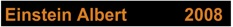
\includegraphics[width=75mm]{Buchruecken}
%\caption[Beschriftung eines Buchr"uckens.]{Beispiel f"ur die Beschriftung eines
%Buchr"uckens.}\label{Abb1}
%\end{figure}
%%Tabelle~\ref{Tab1} ist ein Beispiel daf"ur, wie eine Tabelle aussehen k"onnte.
%\begin{table}[htbp]
%\centering
%\begin{tabular}{ | c | c | c | }\hline
%{\bf Datum} & {\bf Thema} & {\bf Raum}\\ \hline
%\hline
%20. 08. 2008 & Graphentheorie & HS 3.13\\ \hline
%01. 10. 2008 & Biomathematik & HS 1.05\\ \hline
%\end{tabular}
%\caption[Semesterplan "`Angewandte Mathematik"'.]{Beispiel f"ur einen
%Semesterplan "`Angewandte Mathematik"'.}\label{Tab1}
%\end{table}

%\noindent
%Nun ein Beispiel f"ur eine abgesetzte Formel:
%\begin{equation}
%x =  - \frac{p}{2} \pm \sqrt{\left(\frac{p}{2}\right)^2 - q}.
%\end{equation}
%Und eine mehrzeilige Formel:
%\begin{eqnarray}
%f(t)&=& t^2 \label{For1},\\
%g(t) &=& t-1.
%\end{eqnarray}
%Hier wird auf die Formel (\ref{For1}) verwiesen. \\

%\noindent
%So kann zum Beispiel ein \glqq Source-Code\grqq\  angegeben werden: 
%\begin{verbatim}
%for (i=1; i < 10; i++) {...} 
%\end{verbatim}

%\noindent
%Hier ist ein Hyperlink auf die  \href{http://www.technikum-wien.at}{Homepage}
%der FH Technikum Wien. Email-Adressen k"onnen so verlinkt werden:
%\href{mailto:homer.simpson@springfield.com}{\texttt{
%homer.simpson@springfield.com}}\\

%\noindent
%In der Bibliothek der Fachhochschule Technikum Wien gibt es verschiedene
%einf"uhrende B"ucher zum Thema \glqq \LaTeX \grqq, zum Beispiel \cite{kop05},
%\cite{wil06} oder \cite{mgb+05d} (deutsche Version) bzw. \cite{mgb+04e}
%(englische Version). Empfehlenswerte Skripten f"ur \LaTeX-Einsteiger sind z.B.
%\cite{mj00} und \cite{mj95}. Sie sind frei im Internet verf"ugbar.



% Literaturverzeichnis
% Das Literaturverzeichnis kann auch nach einem allf"alligen Anhang positiioniert werden (siehe "`Leitfaden f"ur Bachelor- und Diplomarbeiten"', Version 2.0, Abschnitt 2.9).

% M"oglichkeit 1: Erzeugung des Literaturverzeichnisses mit BibTeX:
% Die Quellen sind in der Datei *.bib (hier Literatur.bib) einzugeben. Danach muss diese Vorlage einmal geTeXt werden, dann BibTeX angewendet werden und 
% anschliessend nochmals zweimal geTeXt werden.
% Im Text erfolgt die Zitierung mit dem Anker-Schl"usselwort, z.B. \cite{kop05}.
\bibliographystyle{IEEEtran}
\bibliography{Literatur}

% M"oglichkeit 2: Erzeugung eines Literaturverzeichnisses ohne BibTeX:
%\begin{thebibliography}{99}
%\bibitem[kop05]{kop05}
%H.~Kopka, {\em LaTeX, Band 1: Einf"uhrung}, Pearson Studium, M"unchen, 3.~Auflage, 2005.
%\bibitem[knu98]{knu98}
%F.~Mittelbach, M.~Goossens, J.~Braams, D.~Carlisle, and Ch. Rowley, {\em The LaTeX Companion}, 
%Addison-Wesley, 2nd edition, 2004.
%\end{thebibliography}

% Abbildungsverzeichnis
\listoffigures
\addcontentsline{toc}{chapter}{Abbildungsverzeichnis} % f"ugt den Eintrag "Abbildungsverzeichnis" im Inhaltsverzeichnis hinzu
\newpage

% Tabellenverzeichnis
%\listoftables 
%\addcontentsline{toc}{chapter}{Tabellenverzeichnis} % f"ugt den Eintrag
%"Tabellenverzeichnis" im Inhaltsverzeichnis hinzu
%\newpage

% Abk"urzungsverzeichnis
% Bei Verwendung der Dokumentklasse "scrartcl" ist der Befehlt \addchap{Abk"urzungsverzeichnis} durch 
% \addsec{Abk"urzungsverzeichnis} zu ersetzen
\addchap{Abk"urzungsverzeichnis}
\hspace{-17mm}\begin{tabular}{>{\raggedleft}p{0.2\linewidth} p{0.75\linewidth} p{0.1\linewidth}}

www & World Wide Web\\
W3C & World Wide Web Consortium\\
URL & Uniform Resource Locator\\
ARIA & Accessible Rich Internet Applications\\
WAI & Web Accessibility Initiative\\
AJAX & Asynchronous JavaScript and XML\\
BITV & Barrierefreie  Informationstechnologie Verordnung\\
\end{tabular}

% Anh"ange
%\begin{appendix}
%\chapter[Erster Anhang]{"Uberschrift des ersten Anhangs}

%Text Text Text Text Text Text Text Text Text Text Text Text Text Text Text Text
%\end{appendix}

\end{document}
